\documentclass{uofa-eng-assignment}
\usepackage{caption}
\usepackage{subcaption}
\usepackage{hyperref}
\usepackage{float}
\hypersetup{
    colorlinks = false,
    linkbordercolor = {white},
}
\captionsetup[table]{name=Tabla, labelsep=period}
\captionsetup[figure]{name=Figura, labelsep=period}

\newcommand{\hpl}{\hyperlink}
\newcommand{\hpt}{\hypertarget}
\newcommand*{\name}{Joan Sebastian Ramirez Sanchez  }
\newcommand*{\id}{202223948}
\newcommand*{\course}{Control óptimo aplicado a modelos biológicos}
\newcommand*{\assignment}{Reporte de laboratorio 6}
\newcommand*{\dated}{\today}
\newcommand{\tf}{\textbf}

\begin{document}

\maketitle
\section*{Introducción}

Este laboratorio estudia un problema de \textbf{control óptimo aplicado a la explotación de una población de peces}. Se considera una población de peces introducida en un estanque o zona de pesca artificial, donde no existe reproducción durante el período de estudio. El objetivo es determinar una estrategia de cosecha que maximice el beneficio obtenido por la pesca.

La población de peces se representa mediante una variable de estado $x(t)$, que describe el número de peces en el tiempo. Además, se supone que la masa promedio de cada pez aumenta con el tiempo según
\[
f_{mass}(t) = \frac{kt}{t + 1},
\]
donde $k$ representa la masa máxima promedio que puede alcanzar la especie.

La dinámica de la población está dada por
\[
x'(t) = -(m + u(t))x(t),
\]
La ecuación indica que la población disminuye debido tanto a la mortalidad natural como a la actividad pesquera, dónde: 
\begin{itemize}
    \item $m$ es la tasa natural de mortalidad,
    \item $u(t)$ es la tasa de pesca o cosecha,
    \item $0 \le u(t) \le M$.
    \item  \(M\): límite superior de la tasa de cosecha, el cual representa restricciones físicas o tecnológicas asociadas a la actividad pesquera. La condición \(0 \leq u(t) \leq M\) garantiza que la extracción no pueda superar la capacidad máxima disponible. 
    \item \(T\): horizonte temporal de planificación sobre el cual se busca maximizar el beneficio total obtenido por la cosecha. 
    \item \(A\): parámetro asociado a la importancia del crecimiento de los peces dentro del proceso de optimización. Valores más altos de este parámetro favorecen estrategias que permiten a los peces crecer durante más tiempo antes de ser capturados.
\end{itemize}
El problema de control óptimo consiste en maximizar
\[
J = A*\int_{0}^{T} \frac{kt}{t + 1}x(t)u(t) - u(t)^2 \, dt.
\]
El primer término representa el beneficio obtenido por la pesca, pues depende de la cantidad de peces capturados y de su masa promedio. El segundo término modela el costo asociado al esfuerzo de pesca. 

\newpage
\section*{Simulaciones y resultados}
Nuestro caso base se simula con los siguientes parámetros:
\begin{align*}
    A = 5,\quad k = 10,\quad  m = 0.2, \quad x_0 = 0.4, \quad M = 1, \quad T = 10.
\end{align*}
Nos da las siguientes gráficas:
\begin{figure}[h!]
    \centering
    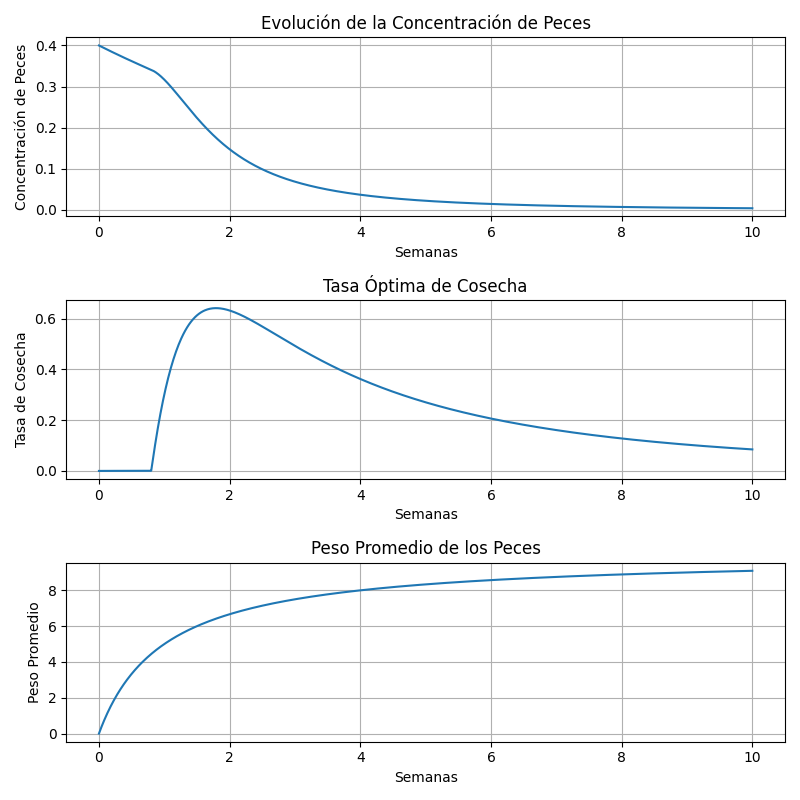
\includegraphics[width=0.5\linewidth]{pa1.png}
    \caption{Simulación del problema de control óptimo para la explotación de una población de peces.}
\end{figure}

La gráfica muestra la evolución de la concentración de peces, la tasa óptima de cosecha y el peso promedio de los peces para los parámetros base del modelo. Inicialmente, la tasa de cosecha permanece cercana a cero durante aproximadamente la primera semana. Este comportamiento indica que la estrategia óptima consiste en permitir que los peces aumenten su peso antes de comenzar la extracción. Durante este período, el peso promedio crece rápidamente mientras la población disminuye únicamente debido a la mortalidad natural. Posteriormente, la tasa de cosecha aumenta de manera pronunciada hasta alcanzar un máximo cercano a (0.6) alrededor de la semana (1.8). Este instante coincide con el momento en que el peso promedio de los peces ha alcanzado un valor suficientemente alto para hacer rentable la cosecha. Después del máximo, la tasa de cosecha disminuye gradualmente. A medida que la población disponible se reduce, resulta menos conveniente mantener una extracción elevada. Como consecuencia, la concentración de peces presenta una disminución continua durante todo el horizonte temporal, acercándose a cero hacia el final de la simulación. Por otra parte, el peso promedio aumenta de forma monótona y parece aproximarse al valor máximo establecido por el parámetro (k=10). Este comportamiento refleja que los peces continúan creciendo durante todo el período analizado. Los resultados obtenidos concuerdan con la interpretación biológica del problema: la estrategia óptima retrasa la cosecha para aprovechar el crecimiento de los peces y posteriormente incrementa la extracción cuando el beneficio asociado al peso de los individuos compensa el costo del esfuerzo de pesca.
\subsection*{Variación de el limite máximo de cosecha}
Para estas simulaciones se modificara el límite máximo de cosecha a $M=0.6$ y $M=0.4$.
\begin{figure}[h!]
    \centering
    
    \begin{subfigure}{0.48\textwidth}
        \centering
        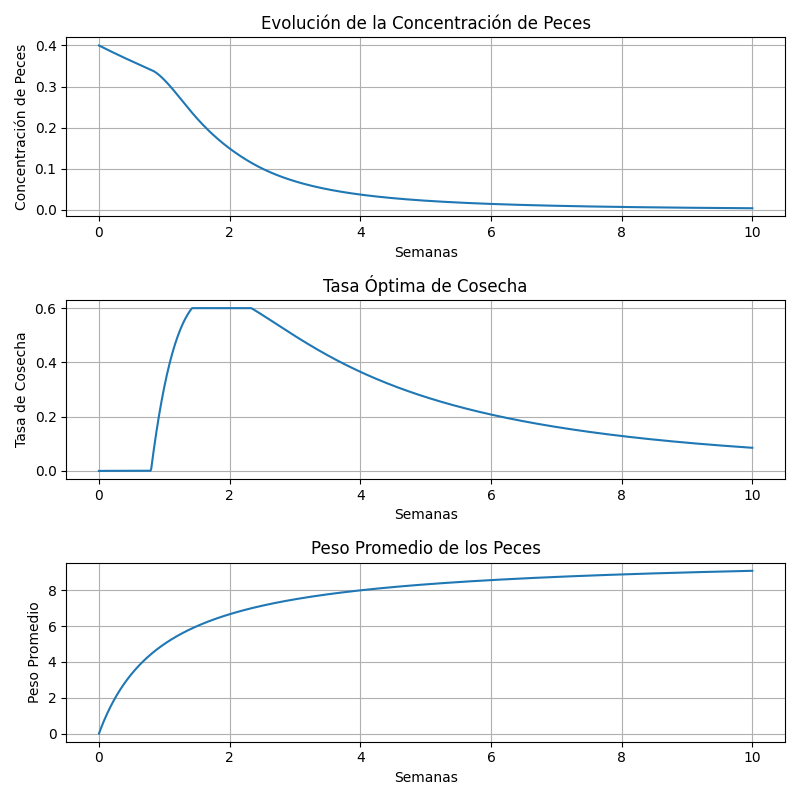
\includegraphics[width=\linewidth]{pa4.png}
        \caption{$M=0.6$}
    \end{subfigure}
    \hfill
    \begin{subfigure}{0.48\textwidth}
        \centering
        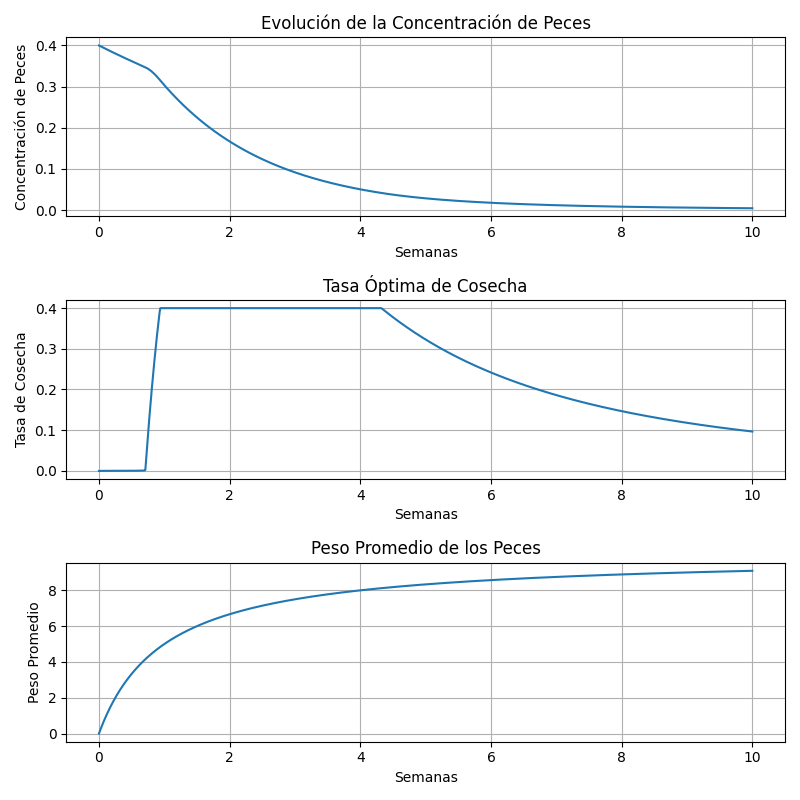
\includegraphics[width=\linewidth]{pa5.png}
        \caption{$M=0.4$}
    \end{subfigure}
    
    \caption{Comparación de las simulaciones para distintos valores de \(M\).}
    \label{fig:comparacion_M}
\end{figure}
Al observar las gráficas, se puede apreciar la cosecha sigue una dinámica similar pero dado que la reducción del limite máximo de la cosecha esto nos permitira cosechar por mas tiempo al máximo y entre más bajo sea este más semanas podremos cosechar al máximo, esto se refleja en el peso promedio de los peces ya que al poder cosechar por más tiempo al máximo esto nos permite tener un peso promedio más alto,
como podemos ver en el caso  ($m=0.4$) podemos cosechar al máximo antes de que la población disminuya y asi aprovechar pescados con mayor peso, en comparación del caso de ($m=0.6$), donde al cosechar al máximo hace que la población disminuya más rápido y no podamos aprovechar el peso de los peces.
\subsection*{Variación de el parámetro A}
Para esta simulación se modificara el parámetro A a $A=10$

\begin{figure}[H]
    \centering
    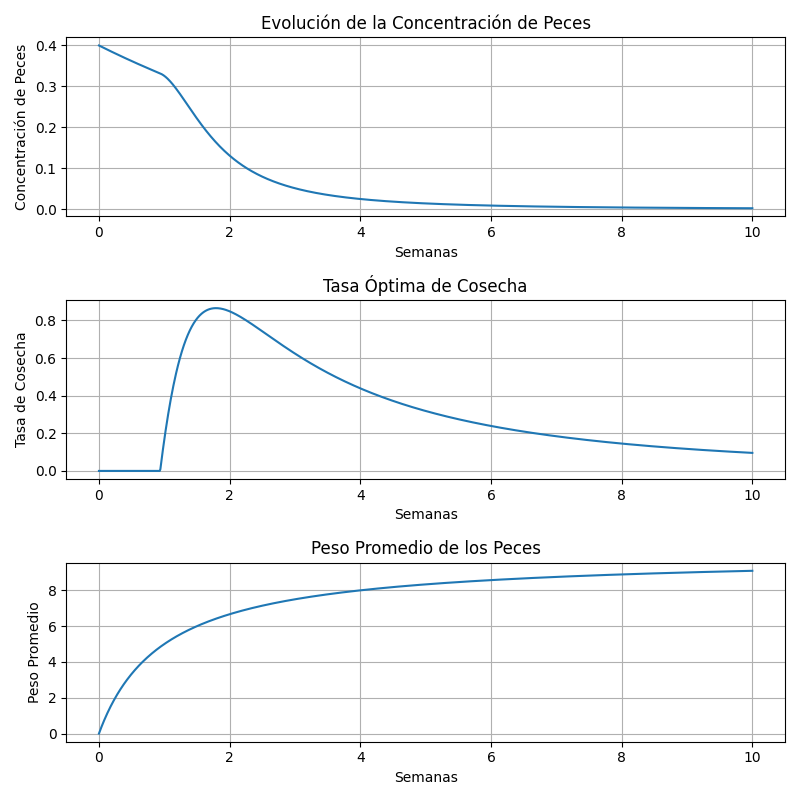
\includegraphics[width=0.4\linewidth]{pa6.png}
    \caption{Simulación del problema de control óptimo para la explotación de una población de peces con \(A=10\).}
\end{figure}
Al aumentar el parámetro $A$ de (5) a (10), no se observaron cambios significativos en las trayectorias de la población ni en la estrategia óptima de cosecha. Aunque este parámetro incrementa la importancia del beneficio asociado al peso de los peces dentro del funcional objetivo, para los valores considerados en el experimento dicho aumento no fue suficiente para modificar de manera apreciable la solución óptima. Esto sugiere que la estrategia obtenida en el caso base ya favorece el crecimiento de los peces antes de la cosecha, por lo que incrementar la ponderación del beneficio no produce variaciones importantes en la dinámica del sistema.
pero se espera que para valores de (A), pasado ciertas semanas la pesca se realice al máximo o sea mayor por más tiempo y así aprovechar el peso y ganancia de los peces.
\subsection*{Variación de la tasa de mortalidad}
Para la siguiente simulación se modificara la tasa de mortalidad natural a $m= 0.6$ y $m=0.4$.
\begin{figure}[h!]
    \centering
    
    \begin{subfigure}{0.48\textwidth}
        \centering
        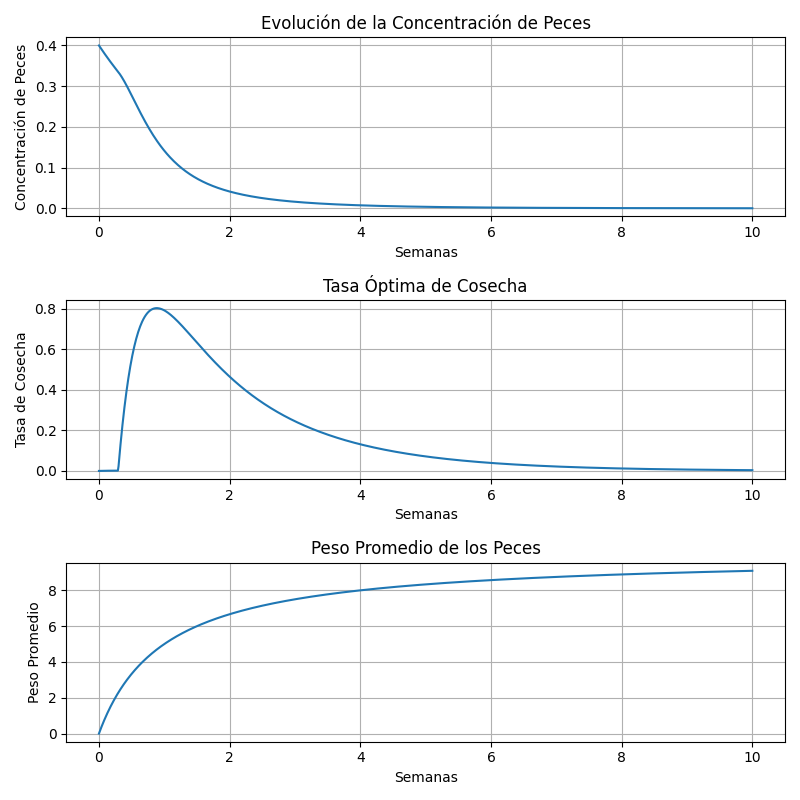
\includegraphics[width=\linewidth]{pa2.png}
        \caption{$m=0.6$}
    \end{subfigure}
    \hfill
    \begin{subfigure}{0.48\textwidth}
        \centering
        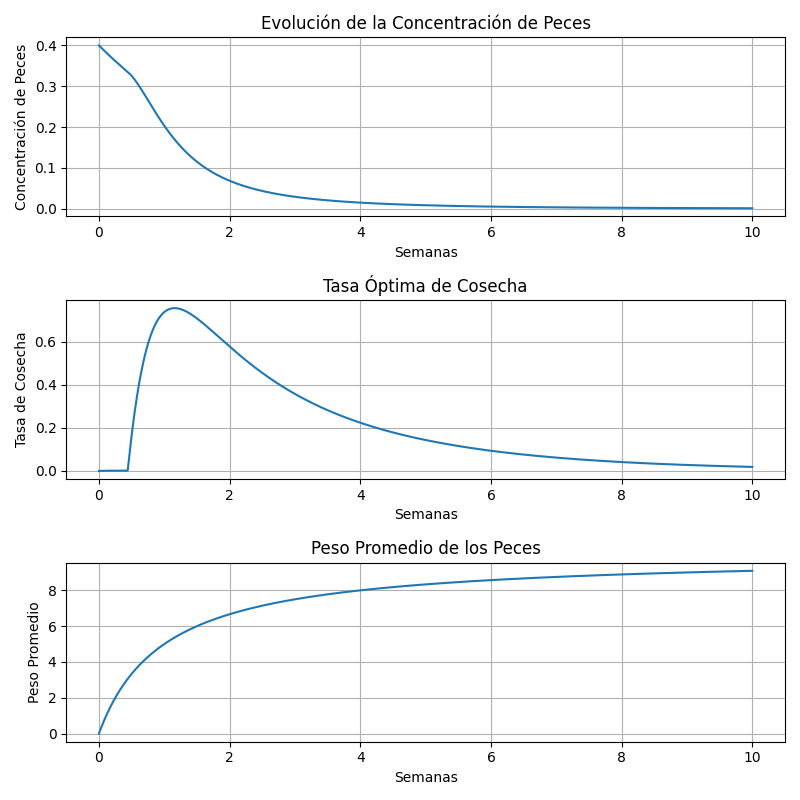
\includegraphics[width=\linewidth]{pa3.png}
        \caption{$m=0.4$}
    \end{subfigure}
    
    \caption{Comparación de las simulaciones para distintos valores de \(m\).}
    \label{fig:comparacion_m}
\end{figure}
Como podemos ver en las graficas la tasa de mortalidad natural tiene un impacto significativo en la dinámica de la población y en la estrategia óptima de cosecha. Para \(m=0.6\), la población de peces disminuye más rápidamente debido a la mayor mortalidad, lo que resulta en una tasa de cosecha más baja y un peso promedio que no alcanza valores tan altos como en el caso con \(m=0.2\). En contraste, para \(m=0.4\), la población se mantiene más estable durante un período más largo, permitiendo una tasa de cosecha más alta y un peso promedio que se acerca más al valor máximo establecido por \(k\). Estos resultados resaltan la importancia de considerar la tasa de mortalidad natural al diseñar estrategias de explotación sostenible para poblaciones biológicas.
\newpage
\subsection*{Variación de la población inicial}
Haciendo una variación de la población inicial de los parámetros base a $x_0=0.8$ tenemos que 
\begin{figure}[h!]
    \centering
    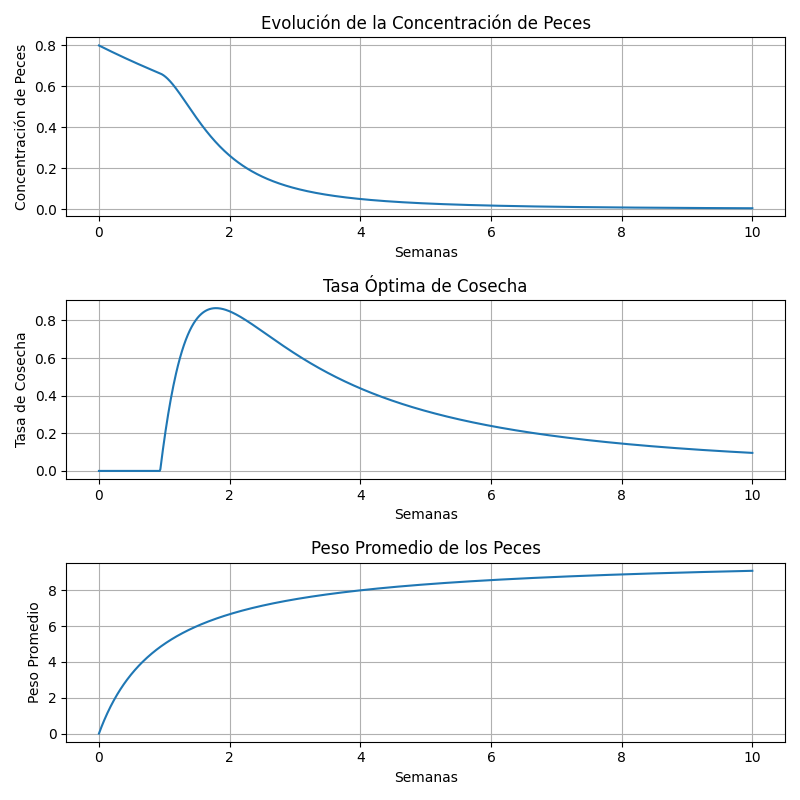
\includegraphics[width=0.5\linewidth]{pa7.png}
    \caption{Simulación del problema de control óptimo para la explotación de una población de peces con \(x_0=0.8\).}
\end{figure}
\\
Podemos ver que un aumento ligero en la población inicial de peces no produce cambios significativos en la dinámica del sistema ni en la estrategia óptima de cosecha. La trayectoria de la población y el peso promedio siguen un comportamiento similar al caso base, aunque con una ligera diferencia en los valores absolutos debido a la mayor cantidad de peces disponibles al inicio. Esto sugiere que, dentro del rango considerado, la solución óptima es robusta frente a variaciones moderadas en la población inicial. 
\subsection*{Comparaciones con el tiempo final}
Para finalizar, se compararan las simulaciones para distintos tiempos finales, $T=10$ y $T=5$.
\begin{figure}[h!]
    \centering
    
    \begin{subfigure}{0.48\textwidth}
        \centering
        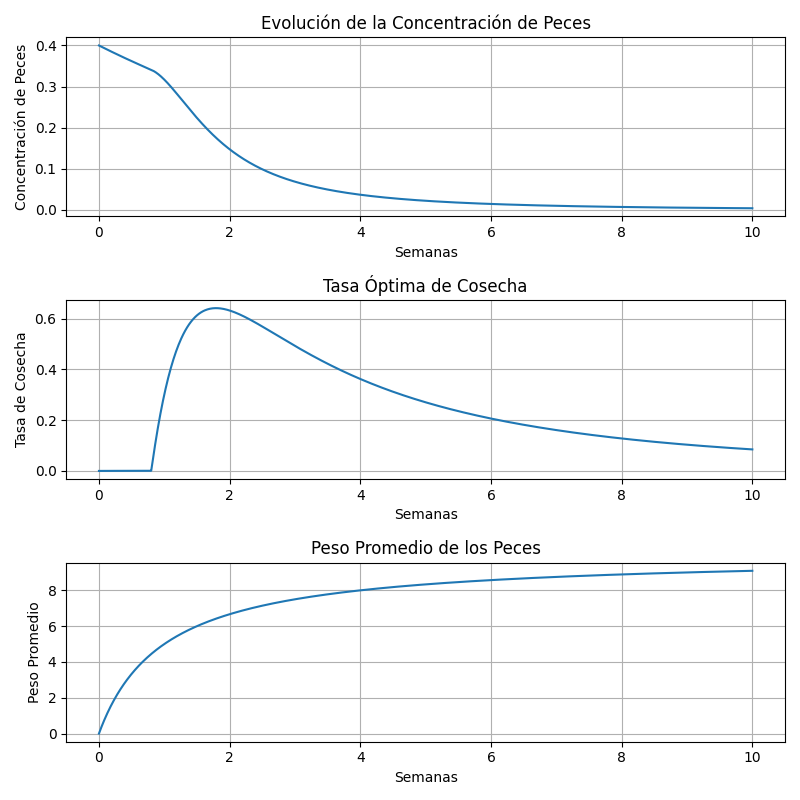
\includegraphics[width=\linewidth]{pa1.png}
        \caption{$T=10$}
    \end{subfigure}
    \hfill
    \begin{subfigure}{0.48\textwidth}
        \centering
        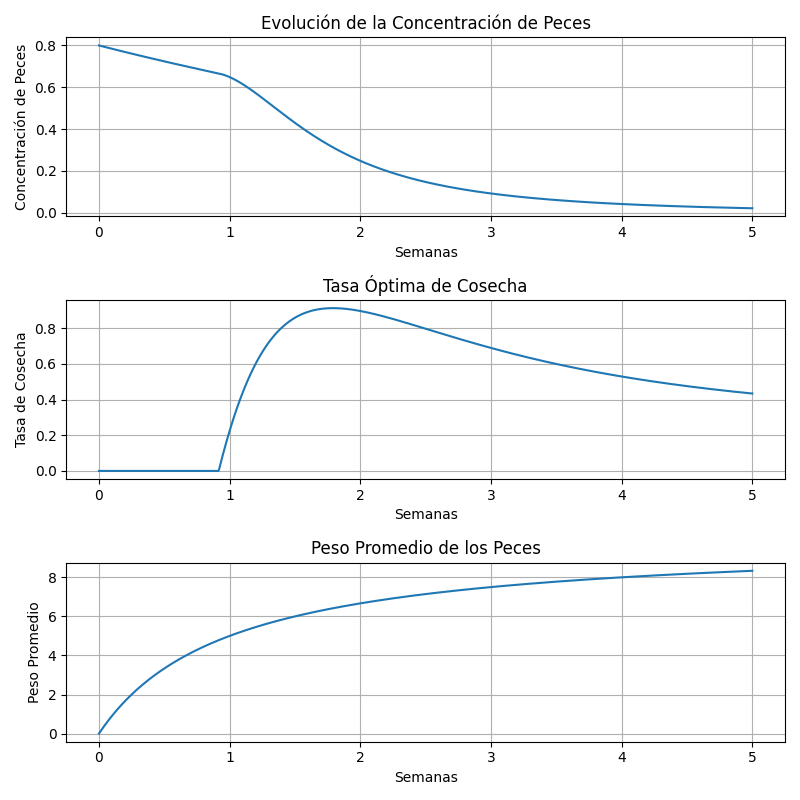
\includegraphics[width=\linewidth]{pa9.png}
        \caption{$T=5$}
    \end{subfigure}
    
    \caption{Comparación de las simulaciones para distintos valores de \(T\).}
    \label{fig:comparacion_T}
\end{figure}
\begin{figure}[h!]
    \centering
    
    \begin{subfigure}{0.48\textwidth}
        \centering
        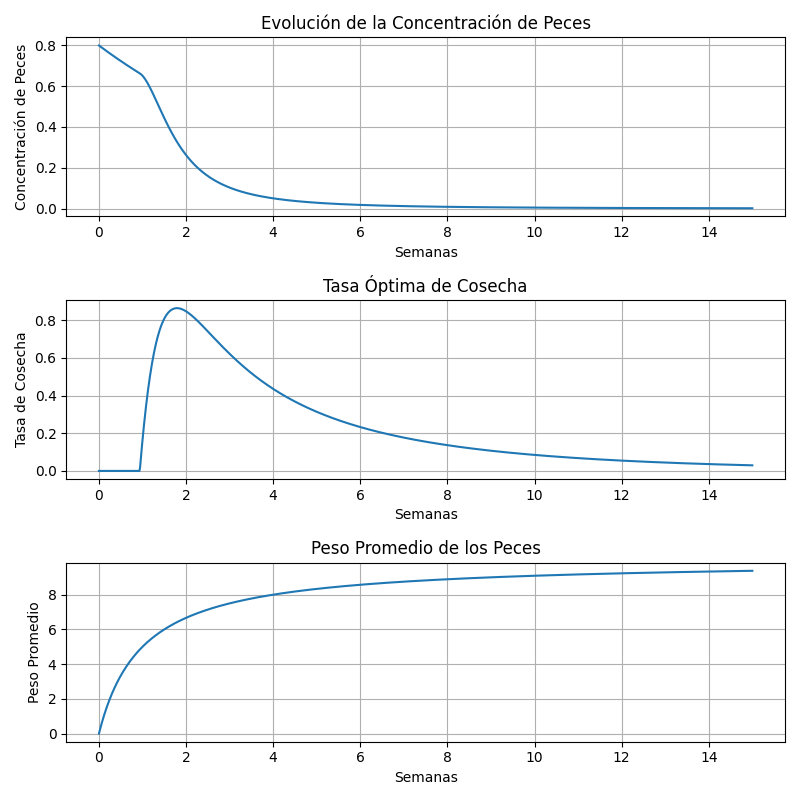
\includegraphics[width=\linewidth]{pa10.png}
        \caption{$T=15$}
    \end{subfigure}
    \hfill
    \begin{subfigure}{0.48\textwidth}
        \centering
        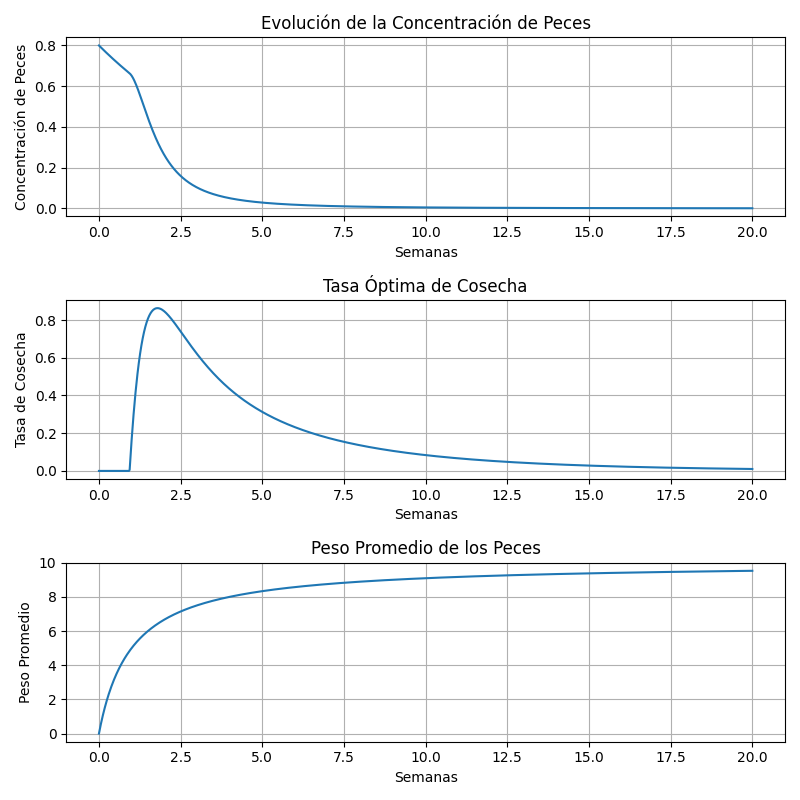
\includegraphics[width=\linewidth]{pa11.png}
        \caption{$T=20$}
    \end{subfigure}
    
    \caption{Comparación de las simulaciones para distintos valores de \(T\).}
    \label{fig:comparacion_T}
\end{figure}

Observe que el tiempo final nos da oportunidad de que tan pronto o cuanto podemos esperar antes de comenzar a cosechar, por ejemplo en el caso de $T=5$ podemos ver que la tasa de cosecha comienza a aumentar antes que en el caso de $T=10$, esto se debe a que al tener un tiempo final más corto nos da menos oportunidad de esperar a que los peces crezcan y así aprovechar su peso, por lo tanto la estrategia óptima es comenzar a cosechar antes. En contraste, para $T=15$ se observa que la tasa de cosecha permanece cerca de cero durante un período más largo, lo que indica que la estrategia óptima retrasa la extracción para permitir un mayor crecimiento de los peces antes de comenzar la cosecha. Estos resultados resaltan la importancia del horizonte temporal en el diseño de estrategias de explotación sostenible, ya que influye directamente en el momento óptimo para iniciar la actividad pesquera y maximizar el beneficio obtenido.
\end{document}
